\chapter{Fizikai modell}\label{chap:physical_system}

\section{Egyenáramú motor dinamikája}

\begin{figure}[ht]
\begin{center}
\phantomsection{}
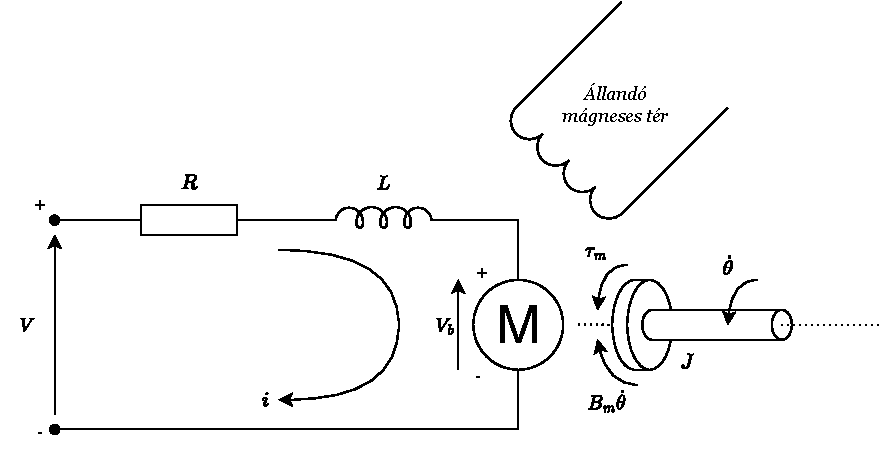
\includegraphics[width=\textwidth]{images/dc_motor_model.pdf}
\caption{Egyenáramú motor áramkör és szabadtest ábra}
\label{fig:dc_motor}
\end{center}
\end{figure}

A robot motorjának modelljét az~\ref{fig:dc_motor}-es ábra mutatja. A felhasznált motor feltételezetten állandó gerjesztésű. A kifejtett nyomaték 
a Biot-Savart-törvény szerint arányos a forgórészen átfolyó árammal. A forgórészben
indukált feszültség pedig arányos annak szögsebességével. A Lenz-törvény alapján 
\begin{align}
    \tau_m = K_\tau i, \\
    V_b = K_e \dot\theta,
\end{align}
ahol $K_\tau$ a nyomatékállandó, $K_e$ a sebesség-feszültség állandó, $\tau_m$ a kifejtett 
nyomaték, $i$ a rotor árama, $V_b$ az rotorban indukált feszültség és $\dot\theta$ a rotor szögsebessége.
Az energia-megmaradás törvénye alapján a két konstans értéke megegyezik
\begin{align}
    K_m = K_\tau = K_e,
\end{align}
így a következőkben $K_m$ paraméterként jelennek meg. A forgórész áramkörére Kirchhoff I. törvénye alapján felírható
\begin{align}\label{eq:armature_circuit}
    V - Ri - L\frac{di}{dt} - K_m\dot\theta = 0,
\end{align}
ahol $R$ a forgórész tekercsének ellenállása, $L$ a tekercs induktivitása, 
$K_m$ a motorállandó, $V$ a motor feszültsége, $i$ a motoráram és $\theta$ a szögelfordulás.
A forgórészt mechanikailag egy merev testként tekintve Newton II. törvénye alapján
\begin{align}\label{eq:rotor_dynamics}
    J\ddot\theta = -B_m\dot\theta + K_m i + \tau,
\end{align}
ahol $J$ a forgórész tehetetlensége, $B_m$ a viszkózus csillapítási együttható, 
$K_m$ a motorállandó, $\theta$ a szögelfordulás, $i$ a motoráram és $\tau$ a forgórészre
ható külső nyomaték. Ez a két lineáris differenciálegyenlet egyértelműen leírja a 
rendszer időtartománybeli viselkedését.
A további vizsgálathoz kedvezőbb a differenciálegyenleteket állapottér modellként felírni.
Egy állapottér modell általánosan
\begin{align}\label{eq:state_space_generic}
    \dot{\bm x} = \bm A \bm x + \bm B \bm u
\end{align}
\begin{align}\label{eq:state_space_generic_out}
    y = \bm C \bm x + \bm D \bm u
\end{align} 
alakban írható fel. 
A két bemenet a külső nyomaték és a motorra adott feszültség. A kimenet a forgórész szöge.
A paramétereket kifejtve~\eqref{eq:armature_circuit} és~\eqref{eq:rotor_dynamics} alapján a modell
\begin{align}\label{eq:state_space}
    \frac{d}{dt}
    \begin{bmatrix}
        \theta \\
        \dot\theta \\
        i
    \end{bmatrix}
    =
    \begin{bmatrix}
        0 & 1 & 0 \\
        0 & -\frac{B_m}{J} & \frac{K_m}{J} \\
        0 & -\frac{K_m}{L} & -\frac{R}{L} \\
    \end{bmatrix}
    \begin{bmatrix}
        \theta \\
        \dot\theta \\
        i
    \end{bmatrix}
    +
    \begin{bmatrix}
        0 & 0 \\
        \frac{1}{J} & 0 \\
        0 & \frac{1}{L} \\
    \end{bmatrix}
    \begin{bmatrix}
        \tau \\
        V \\
    \end{bmatrix}
\end{align}
\begin{align}\label{eq:state_space_out}
    \theta = 
    \begin{bmatrix}
        1 & 0 & 0
    \end{bmatrix}
    \begin{bmatrix}
        \theta \\
        \dot\theta \\
        i
    \end{bmatrix}
    +
    \begin{bmatrix}
        0 & 0
    \end{bmatrix}
    \begin{bmatrix}
        \tau \\
        V \\
    \end{bmatrix}
\end{align}
alakba írható át. A frekvenciatartománybeli vizsgálatokhoz felírható a rendszer 
szög-nyomaték és szög-feszültség átviteli függvénye. Az állapottér modellt felhasználva
\begin{align}\label{eq:transfer_generic}
    \frac{Y(s)}{U(s)} = \bm C{\left(s \bm I - \bm A\right)}^{-1} \bm B + D
\end{align}
általános formában, ahol $\bm I$ az identitás mátrix. Behelyettesítve~\eqref{eq:state_space} és~\eqref{eq:state_space_out}
paramétereit~\eqref{eq:transfer_generic} felírható
\begin{align}\label{eq:transfer_function}
    \begin{bmatrix}
        \frac{\theta(s)}{\tau(s)} \\ 
        \frac{\theta(s)}{V(s)} \\ 
    \end{bmatrix}
    =
    \frac{1}{s\left(JLs^2 + \left(B_m L + JR\right)s + K_m^2 + B_m R\right)}
    \begin{bmatrix}
        Ls + R \\ 
        K_m \\ 
    \end{bmatrix}
\end{align}
alakban.

\section{Egyenáramú motor stabilitása}
A szabályozókör visszacsatoló ágának megbomlása instabilitáshoz vezet, ha a 
szabályozó vagy a szabályozott rendszer önmagában instabil. Ez a valós rendszernél 
szaturációt eredményez, mely a jelen alkalmazás kontextusában nem elfogadható. A motor stabilitása ezért 
egy rendszerkövetelmény, ami a karakterisztikus egyenletből meghatározható.
Az~\eqref{eq:transfer_function}-es átviteli függvény alapján a karakterisztikus egyenlet
\begin{align}
    JLs^2 + \left(B_m L + JR\right)s + K_m^2 + B_m R = 0,
\end{align}
ahol a nullában elhelyezkedő pólussal átszorozva a szögsebesség a vizsgált kimenet.
Ez a polinom valós együtthatókkal rendelkezik, így a Liénard–Chipart kritérium - a Routh-Hurwitz kritérium módosított
alakja - segítségével a stabilitás szükséges és elégséges feltételei
\begin{align}
    JL>0,\quad B_m L + JR > 0,\quad K_m^2 + B_m R > 0.
\end{align}
A feltételekben megjelenő paraméterek mind pozitívak a valós rendszerben, így a rendszer
önmagában aszimptotikusan stabil. Ezen felül linearitásából következik, hogy exponenciálisan stabil.

\section{Irányíthatóság és megfigyelhetőség}
A felhasznált aktuátorok és szenzorok minimalizálása érdekében egy bemenet és egy kimenet használata a cél. 
Az impedancia modell teljes realizálásához további követelmény, hogy a rendszer szögelfordulása és szögsebessége
irányítható legyen a bemeneti feszültség megváltoztatásával, és a szögelfordulás mérésével minden állapot 
megfigyelhető legyen. Az~\eqref{eq:state_space_generic}-os állapottér modell alapján az irányíthatóság feltétele, hogy
\begin{align}
    \left[\begin{array}{c|c|c|c}
        \bm{CB} & \bm{CAB} & \bm C \bm A^2 \bm B & \bm D
    \end{array}\right]
\end{align}
legyen maximális rangú. Behelyettesítve~\eqref{eq:state_space} és~\eqref{eq:state_space_out} paramétereit a kimeneti mátrixot kiegészítve a szögsebességgel
\begin{align}
    \begin{bmatrix}
        0 & 0 & \frac{K_m}{JL} & 0 \\
        0 & \frac{K_m}{JL} & -\frac{K_m\left(B_m L + JR\right)}{J^2L^2} & 0
    \end{bmatrix},
\end{align}
redukált lépcsős alakban
\begin{align}
    \begin{bmatrix}
        0 & 1 & 0 & 0 \\
        0 & 0 & 1 & 0
    \end{bmatrix},
\end{align}
mely mátrix rangja megegyezik sorainak számával, így az irányíthatósági feltétel teljesül. Az előzőekhez hasonlóan a 
megfigyelhetőség feltétele, hogy
\begin{align}
    \left[\begin{array}{c}
        \bm{C} \\ \hline
        \bm{CA} \\ \hline
        \bm C \bm A^2
    \end{array}\right]
\end{align}
legyen maximális rangú, ahol $\bm C$ csupán a szöglfordulást tartalmazza. Ismét behelyettesítve
~\eqref{eq:state_space} és~\eqref{eq:state_space_out} paramétereit
\begin{align}
    \begin{bmatrix}
        1 & 0 & 0 \\
        0 & 1 & 0 \\
        0 & -\frac{B_m}{J} & \frac{K_m}{J}
    \end{bmatrix},
\end{align}
redukált lépcsős alakban
\begin{align}
    \begin{bmatrix}
        1 & 0 & 0 \\
        0 & 1 & 0 \\
        0 & 0 & 1
    \end{bmatrix},
\end{align}
tehát a rendszer minden állapota megfigyelhető a szögelfordulás méréséből.
\chapter{Szabályozó modellezése}\label{chap:controller}

\section{Impedancia modell}
Az eredményes ember-robot interakció érdekében a szabályozó előírása nem csupán 
az elérni kívánt pozíció vagy kifejtett nyomaték, hanem a mozgásállapot és a kifejtett
nyomaték közötti összefüggés. Ezt az összefüggést linearitása végett egy 
tömeg-rugó-csillapitás modell adja meg a továbbiakban. A modell három paraméterrel
\begin{align}
    M_e \ddot \theta + B_e \dot \theta + K_e \theta = \tau,
\end{align}
ahol $M_e$ a rendszer előírt tehetetlensége, $B_e$ a viszkózus csillapítása, $K_e$ a rugóállandója 
és $\tau$ a rendszerre ható külső nyomaték. 
\section{Állapotmegfigyelő}
Az állapotvisszacsatoláshoz szükséges belső állapotok közül csak a szögelfordulás
áll rendelkezésre közvetlen mérésből. A többi állapotra egy megfigyelő ad becslést.
Elkülönítve a mért és becsült állapotokat~\eqref{eq:state_space_generic} és~\eqref{eq:state_space_generic_out} felírható
\begin{align}\label{eq:observer}
    \left[\begin{array}{c}
        \dot\theta \\ \hline
        \dot{\bm x}_b
    \end{array}\right]
    =
    \left[\begin{array}{c|c}
        A_{\theta\theta} & \bm A_{\theta b} \\ \hline
        \bm A_{b \theta} & \bm A_{bb}
    \end{array}\right]
    \left[\begin{array}{c}
        \theta \\ \hline
        \bm x_b
    \end{array}\right]
    +
    \left[\begin{array}{c}
        B_\theta \\ \hline
        \bm B_b
    \end{array}\right]
    \begin{bmatrix}
        \tau \\
        V \\
    \end{bmatrix}
\end{align}
\begin{align}\label{eq:observer_out}
    \theta = 
    \left[\begin{array}{c|c}
        1 & \bm 0
    \end{array}\right]
    \left[\begin{array}{c}
        \theta \\ \hline
        \bm x_b
    \end{array}\right]
\end{align}
alakban, ahol $\bm{x}_b$ jelöli a becsült állapotokat. Továbbá jelölje $\tilde{*}$ 
a becsült paramétereket. Ezután legyen
\begin{align}
    \begin{split}
    \hat{\bm A} &= \bm A_{bb} - \bm K_e \bm A_{\theta b} \\
    \hat{\bm B} &= \hat{\bm A} \bm K_e + \bm A_{b \theta} - \bm K_e A_{\theta \theta} \\
    \hat{\bm F} &= \bm B_b - \bm K_e B_\theta,
    \end{split}
\end{align}
ahol $\hat{\bm A}$ a megfigyelő belső állapotának (továbbiakban $\tilde{\bm \eta}$) 
dinamikáját adja meg, $\hat{\bm B}$ és $\hat{\bm F}$ a mért illetve a becsült állapotok 
bemeneti mátrixai. A becsült állapotok és az állapotváltozók közötti összefüggés ekkor
\begin{align}
    \begin{split}
    \bm \eta = \bm x_b - \bm K_e \theta \\
    \tilde{\bm \eta} = \tilde{\bm x}_b - \bm K_e \theta
    \end{split}
\end{align}
alakban adható meg. A belső állapot dinamikája
\begin{align}
    \begin{split}
    \dot{\tilde{\bm \eta}} = \hat{\bm A} \tilde{\bm \eta} + \hat{\bm B} \theta + \hat{\bm F} u.
    \end{split}
\end{align}
Végül~\eqref{eq:observer_out} átalakításával a rendszer becsült állapotvektora
\begin{align}
    \tilde{\bm x} = \hat{\bm C} \tilde{\bm \eta} + \hat{\bm D} \theta,
\end{align}
ahol
\begin{align}
    \hat{\bm C} = 
    \left[\begin{array}{c}
        \bm 0 \\ \hline
        \bm I_{n-1}
    \end{array}\right],
    \quad
    \hat{\bm D} = 
    \left[\begin{array}{c}
        1 \\ \hline
        \bm K_e
    \end{array}\right],
\end{align}
mely tartalmazza a mért állapotot is.

\section{Nyomaték kompenzáció}
A modell két bemenete közül csak a feszültségre van hatással a 
szabályozó. A külső nyomaték környezeti hatásokból ered. Az impedancia 
modell mindkét bemenetre adott válasz alakját előírja, így a környezet 
hatását a feszültség megváltoztatásával kell kompenzálni. A kompenzáció
a külső nyomaték direkt vagy indirekt visszacsatolásával érhető el.
Direkt mérés esetén a külső nyomaték értékét egy szenzor adja meg, 
mely dinamikája jelen vizsgálat során elhanyagolható. Az
állapotmegfigyelővel és kompenzációval ellátott rendszer teljes 
blokkdiagramját az~\ref{fig:block_diagram_direct_compensation}-es ábra mutatja.
\begin{figure}[ht]
    \begin{center}
    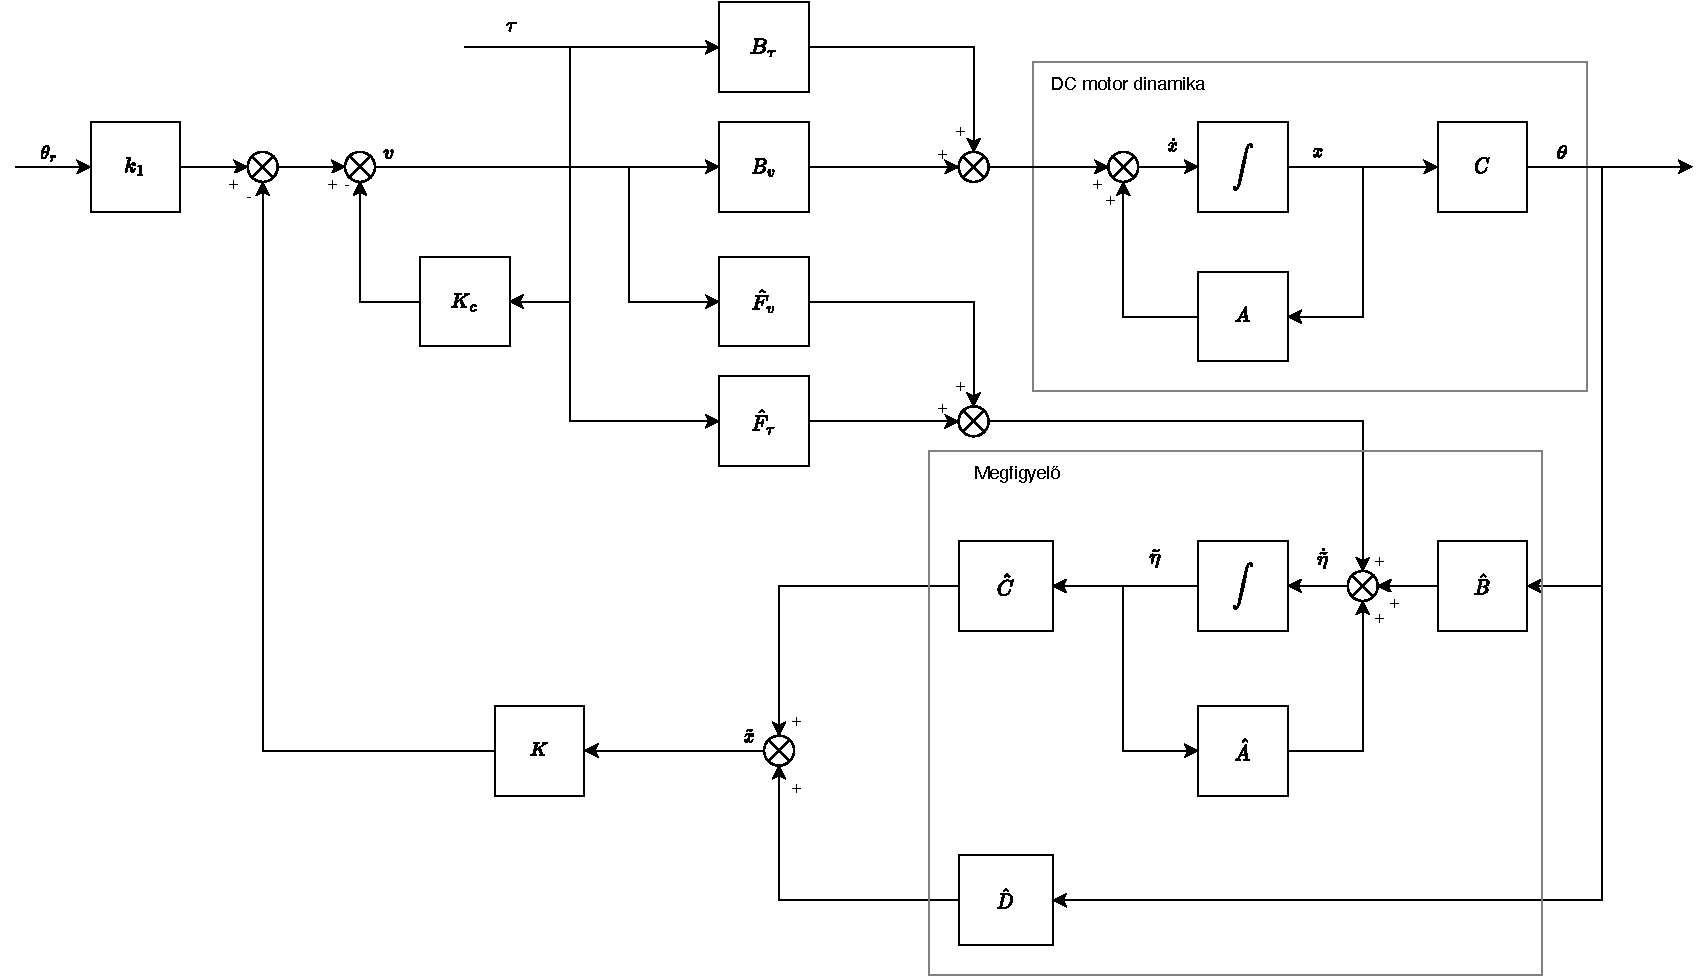
\includegraphics[width=\textwidth]{images/compensated_position_control_torque.drawio.pdf}
    \caption{Impedancia szabályozó közvetlen nyomaték méréssel}\label{fig:block_diagram_direct_compensation}
    \end{center}
\end{figure}
A teljes rendszer dinamikája az~\eqref{eq:state_space}-es állapottér modell és az ~\eqref{eq:observer}-es 
állapotmegfigyelő összekapcsolásával írható le, a következő visszacsatolási összefüggéssel
\begin{align}
    V = -\bm K \tilde{\bm x} -K_c \tau + k_1 \theta_r,
\end{align}
ahol $\bm K$ az állapot visszacsatolási mátrix, $K_c$ a nyomaték kompenzációs együttható,
$k_1$ a az állapot visszacsatolási mátrix első eleme és $\theta_r$ az előírt szögelfordulás.
Behelyettesítve~\eqref{eq:state_space}-ba
\begin{align}\label{eq:state_control_law_subs}
    \dot{\bm x} = \bm A \bm x + \bm B_V\left[-\bm K \tilde{\bm x} -K_c \tau + k_1 \theta_r\right] + \bm B_\tau \tau,
\end{align}
ahol a bemeneti mátrix $\bm B$ oszlopai elkülönítve $\bm B_V$ és $\bm B_\tau$ paraméterként jelennek meg.
Bevezetve a valós és becsült állapot közötti hibát, mint
\begin{align}
    \bm e = \bm x - \tilde{\bm x},
\end{align}
~\eqref{eq:state_control_law_subs} a következő alakra hozható
\begin{align}
    \dot{\bm x} = \left(\bm A - \bm B_V \bm K\right) \bm x + 
    \bm B_V \bm K \bm e + 
    \left(\bm B_\tau - \bm B_V K_c\right) \tau + 
    \bm B_V k_1 \theta_r,
\end{align}
a becsült állapot kiküszöbölésével. A valós és becsült állapot közötti eltérés dinamikája 
pedig~\eqref{eq:observer} felhasználásával
\begin{align}
    \dot{\bm x}_b = \bm A_{b\theta} x_\theta + \bm A_{bb} \bm x_b + 
    \bm B_{bB} V + \bm B_{b\tau} \tau,
\end{align}
\begin{align}
    \dot{\tilde{\bm x}}_b = \left(\bm A_{bb} - \bm K_e \bm A_{\theta b}\right) \tilde{\bm x}_b +
    \bm A_{b\theta} x_\theta +
    \bm K_e \bm A_{\theta b} \bm x_b +
    \bm B_{bB} V + \bm B_{b\tau} \tau,
\end{align}
melyeket kivonva egymásból
\begin{align}
    \dot{\bm e} = \left(\bm A_{bb} - \bm K_e \bm A_{\theta b}\right) \bm e.
\end{align}
A rendszer dinamikája blokk mátrix alakban
\begin{align}
    \begin{bmatrix}
        \dot{\bm x} \\
        \dot{\bm e}
    \end{bmatrix}
    =
    \begin{bmatrix}
        \bm A - \bm B_V \bm K & \bm B_V \bm K \\
        \bm 0 & \bm A_{bb} - \bm K_e \bm A_{\theta b}
    \end{bmatrix}
    \begin{bmatrix}
        \bm x \\
        \bm e
    \end{bmatrix}
    +
    \begin{bmatrix}
        \bm B_\tau - \bm B_V K_c & \bm B_V k_1\\
        \bm 0 & \bm 0
    \end{bmatrix}
    \begin{bmatrix}
        \tau \\
        \theta_r
    \end{bmatrix}.
\end{align}

Indirekt nyomaték visszacsatolás kontextusában, a rendszer szöggyorsulásának mérése alapján,
az~\ref{fig:block_diagram_indirect_compensation}-es ábra mutatja a teljes blokkdiagramot.
\begin{figure}[ht]
    \begin{center}
    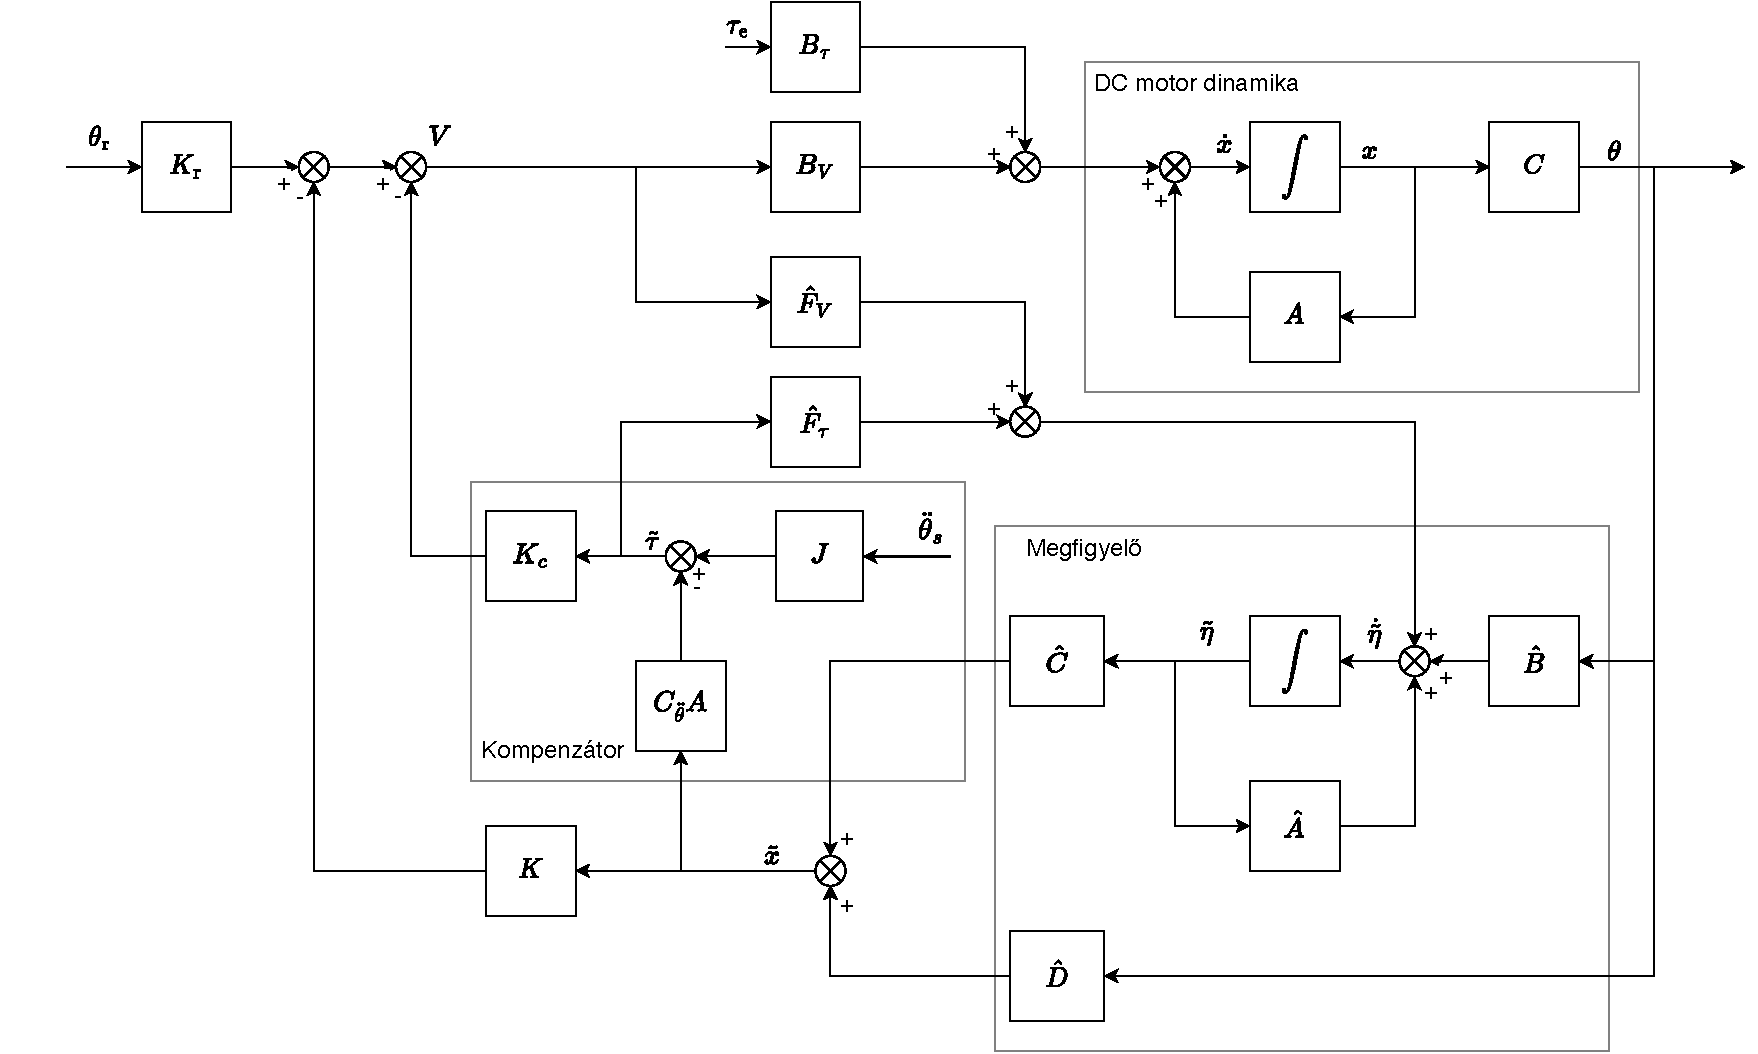
\includegraphics[width=\textwidth]{images/compensated_position_controller_angular_acceleration.pdf}
    \caption{Impedancia szabályozó szöggyorsulás méréssel}\label{fig:block_diagram_indirect_compensation}
    \end{center}
\end{figure}
Ekkor egy becsült nyomaték érték kerül visszacsatolásra, melyeket
\begin{align}
    \tilde \tau = J \ddot \theta_s - \bm C_{\ddot\theta} \bm A \tilde{\bm x}
\end{align}
\begin{align}
    \bm C_{\ddot\theta} = 
    \begin{bmatrix}
        0 & 1 & 0
    \end{bmatrix}
\end{align}
alakban, a becsült állapot és a mért szöggyorsulás kombinációjával adható meg.
A feszültségjel a becsült nyomatékértékkel
\begin{align}
    V = -\bm K \tilde{\bm x} -K_c \tilde \tau + k_1 \theta_r.
\end{align}
Az előző levezetéshez hasonlóan a teljes rendszer dinamikája blokk mátrix alakban
% \begin{align}
%     \begin{bmatrix}
%         \dot{\bm x} \\
%         \dot{\bm e}
%     \end{bmatrix}
%     =
%     \begin{bmatrix}
%         \bm A - \bm B_V \bm K & \bm B_V \bm K \\
%         \bm 0 & \bm A_{bb} - \bm K_e \bm A_{\theta b}
%     \end{bmatrix}
%     \begin{bmatrix}
%         \bm x \\
%         \bm e
%     \end{bmatrix}
%     +
%     \begin{bmatrix}
%         \bm B_\tau - \bm B_V K_c & \bm B_V k_1\\
%         \bm 0 & \bm 0
%     \end{bmatrix}
%     \begin{bmatrix}
%         \tau \\
%         \theta_r
%     \end{bmatrix}.
% \end{align}



Ez a kompenzáció
csak akkor lehet eredményes, ha a rendszer feszültségre és külső nyomatékra 
egyaránt közel azonos sebességgel reagál.
\begin{figure}[ht]
    \begin{center}
    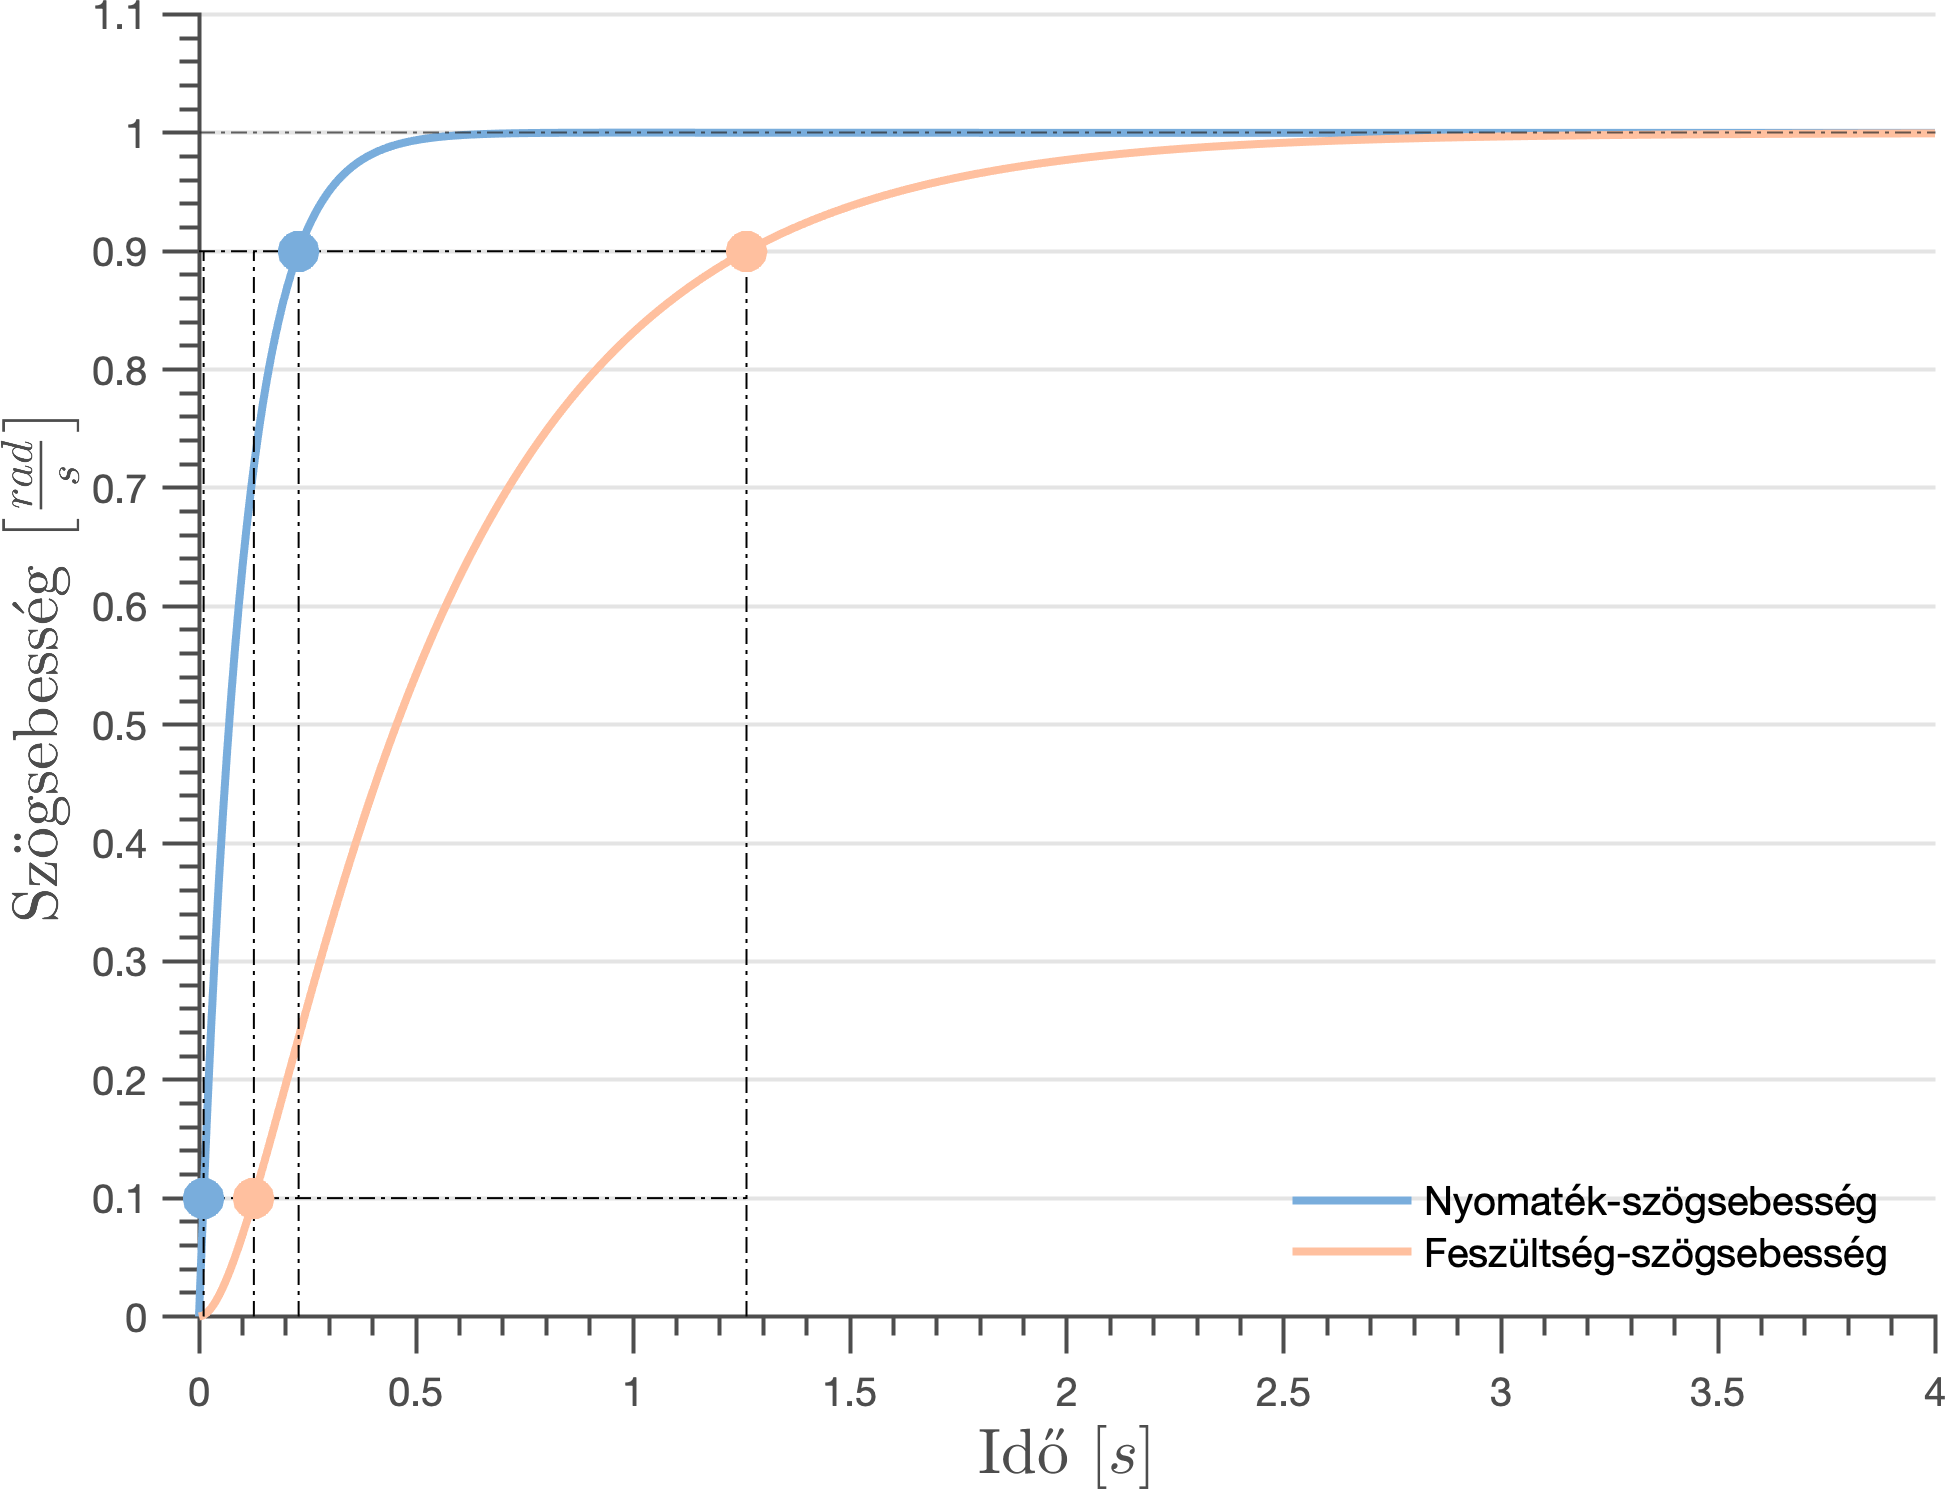
\includegraphics[width=\textwidth]{images/step_response.png}
    \caption{Külső nyomatékra és feszültségre adott válasz összehasonlítása, 
    $J = 0.01 \left[kg\cdot m^2\right]$,
    $K_m = 0.01 \left[kg\cdot \frac{m^2}{s^2}\right]$,
    $B_m = 0.1 \left[kg\cdot \frac{m^2}{s}\right]$,
    $L = 0.5 \left[H\right]$,
    $R = 1 \left[\Omega\right]$}\label{fig:step_response}
    \end{center}
\end{figure}
Az eltérő válaszokat 
szemlélteti~\ref{fig:step_response}-es ábra, mely az~\eqref{eq:transfer_function}-es
egyenletben szereplő átviteli függvények alapján a szögsebesség egységugrásra adott válaszát mutatja. 
A két válasz végértékét egységnyire normalizálva jeleníti meg az ábra a fefutási idő 
összehasonlításának megkönnyítése érdekében. 

\section{Szabályozó stabilitása}

\chapter{Stabilitásvizsgálat időkéséssel}\label{chap:time_delay_stability}

\section{Vizsgálati módszerek összehasonlítása}

\section{Stabilitás folytonos időben}

\section{Stabilitás diszkrét időben}

\chapter{Kísérleti eredmények}\label{chap:experimental_results}

\pagebreak
A rúd differenciálegyenlete
\begin{align}
    \ddot\phi\left(t\right) - \frac{6g}{l}\phi\left(t\right) + 
    \frac{6D}{ml}\dot\phi\left(t-\tau\right) + \frac{6P}{ml}\phi\left(t-\tau\right) = 0
\end{align}
A differenciálegyenlet Laplace transzformáltja
\begin{align}
    s^2\phi\left(s\right) - s\phi_0 - \dot\phi_0 - 
    \frac{6g}{l}\phi\left(s\right) + 
    \frac{6D}{ml}\left(se^{-s\tau}\phi\left(s\right)-\phi_{-\tau}\right) + 
    \frac{6P}{ml}e^{-s\tau}\phi\left(s\right) = 0 
\end{align}
Kifejezve $\phi\left(s\right)$-t
\begin{align}
    \phi\left(s\right) = \frac{s\phi_0+\dot\phi_0+\frac{6D}{ml}\phi_{-\tau}}{s^2+\frac{6D}{ml}se^{-s\tau}+\frac{6P}{ml}e^{-s\tau}-\frac{6g}{l}}
\end{align}
A végérték frekvenciatartománybeli reprezentációban
\begin{align}
    \lim_{t \to \infty}\phi\left(t\right) = 
    \lim_{s \to 0} \phi\left(s\right) = 
    \frac{\dot\phi_0+\frac{6D}{ml}\phi_{-\tau}}{\frac{6P}{ml}-\frac{6g}{l}}
\end{align}
Az időkésést Taylor-sorral közelítve
\begin{align}
    \phi\left(t-\tau\right) = \phi\left(t-\right) - 
    \frac{1}{1!}\dot\phi\left(t\right)\tau + 
    \frac{1}{2!}\ddot\phi\left(t\right)\tau^2 - 
    \frac{1}{3!}\dddot\phi\left(t\right)\tau^3 + \ldots
\end{align}
különböző rendű közelítéssekkel

